%!TEX encoding = UTF-8 Unicode
\documentclass[ % options,
    a4paper,    % papersize
%    cjk,       % for cjk-ko
%    usedotemph,% for cjk-ko's \dotemph
    amsmath,    % load amsmath.sty to typeset math materials
    itemph,     % to disable gremph default (xe/lua)
%    footnote,  % korean style footnote
%    chapter,   % to use \chapter
]{oblivoir}     % xoblivoir and oblivoir are identical.

\ifPDFTeX       % latex, pdflatex
%    \usepackage{newtxtext}    % Latin fonts
\else\ifLuaOrXeTeX   % xelatex or lualatex
%  \setmainfont{TeX Gyre Termes}   %% Latin fonts
%	\setkomainfont(Noto Serif CJK KR)(* Bold)(* Medium)
%	\setkosansfont(Noto Sans CJK KR)(* Bold)(* Medium)
\fi\fi

% color 
\usepackage{xcolor}
\usepackage{titlesec}
\titleformat{\section}{\color{blue}\normalfont\Large\bfseries}{\color{blue}\thesection}{1em}{}
\titleformat{\subsection}{\color{orange}\normalfont\Large\bfseries}{\color{orange}\thesubsection}{1em}{}

% packages
\usepackage{kotex-logo}
\usepackage[utf]{kotex}
\usepackage{geometry}
 \geometry{
 a4paper,
 total={170mm,257mm},
 left=20mm,
 top=20mm,
 }
 
%% font packages and setup
\usepackage{fontspec}
\setmainfont{UnDotum}
\setsansfont{UnDotum}
\setmonofont{UnTaza}
\usepackage{dhucs-interword}
\interhword[.6]{.475}{.1}{.1}
\setlength{\parindent}{0em}
\setlength{\parskip}{1em}

% operator
\DeclareMathOperator*{\argmax}{argmax}
\DeclareMathOperator{\E}{\mathbb{E}}

% image 
\usepackage{graphicx}

% page header
\usepackage{fancyhdr}
\pagestyle{fancy}
\rhead{강화학습}

% box 
\usepackage{tcolorbox}

\begin{document}

\title{강화학습}
\author{wisemountain}
\date{\today}

\maketitle

\newpage

\tableofcontents

\newpage

\section{MDP 개념}

Markov Decision Process가 무엇인지 알아야 강화학습을 시작할 수 있다. 
MDP에 기초하여 MDP 문제를 주어진 환경에서 푸는 것이 강화학습이기 때문이다. 

다양하고 많은 자료들이 있지만 알파고의 제1저자인 데이비드 실버의 
강의 노트가 간결하다. 한글 자료들도 많으므로 함께 읽으면 좋다. 

https://www.davidsilver.uk/wp-content/uploads/2020/03/MDP.pdf


\section{그리드 월드와 다이나믹 프로그래밍}

\subsection{벨만 기대방정식과 최적 방정식}

수식 2.31 벨만 기대 방정식:
$$
v_\pi(s) = \E_\pi[R_{t+1} + \gamma v_\pi(S_{t+1})|S_t = s] 
$$

수식 2.32 계산 가능한 벨만 기대 방정식: 
$$
v_\pi(s) = \sum_{a\in A} \pi(a|s) (R_{t+1} + \gamma \sum_{s' \in S} P_{ss'}^a v_\pi(s'))
$$

수식 2.36 최적의 가치함수: 
$$
v_*(s) = \max_\pi [v_\pi(s)]
$$ 

수식 2.37 최적의 큐함수 (상태행동 가치함수): 
$$
q_*(s, a)= \max_\pi[q_\pi(s,a)]
$$

수식 2.38 최적 정책 :
$$
\pi_*(s, a) = 
	\begin{cases}
		1 \text{ if } a = \underset{a \in A}\argmax q_*(s, a) \\
		0 \text{ otherwise }
	\end{cases}
$$

수식 2.39 큐 함수에 최대를 선택하는 최적 가치함수 :
$$
v_*(s) = \max_a [ q_*(s, a) | S_t = a, A_t = a]
$$

수식 2.40 벨만 최적 방정식 :
$$
v_*(s) = \max_a \E[R_{t+1} + \gamma v_*(S_{t+1}) | S_t = s, A_t = a]
$$

수식 2.41 큐함수에 대한 벨만 최적 방정식 :
$$
q_*(s, a) = \E[R_{t+1} + \gamma \max_{a'} q_*(S_{t+1}, a') | S_t = s, A_t = a]
$$

단단한 강화학습에서 식 2.41을 계산 가능한 형태로 푼 수식은 다음과 같다. 
$$
q_*(s, a) = \sum_{s', r} p(s', r|s, a)[r + \gamma \max_{a'} q_*(s', a')]
$$

여기서 $p(s', r|s, a)$는 $P_{ss'}^{a}$에 r 값 분기가 추가된 것으로 단단한 강화학습에서는 
동일한 행동과 동일한 다음 상태에 대해 서로 다른 보상이 주어지는 분기가 있다고 본다. 

\subsection{다이나믹 프로그래밍} 

큰 문제를 작은 문제로 나누고 작은 문제들을 계산하여 기억한 후
그 값들을 사용하여 큰 문제를 단계적으로 계산하는 최적화 
알고리즘이다. 벨만 방정식(기대, 최적) 모두 재귀적인 형태로 되어 있고 
이전 값을 사용하여 갱신해서 최적 값을 얻는다. 

다이나믹 프로그래밍으로 최적의 정책을 찾아 가는 방법은 두 가지가 있는데 
하나는 정책 이터레이션이고 하나는 가치 이터레이션이다. 두 가지 모두 이터레이션(iteration)을
갖고 있는데 이는 반복적으로 실행하여 최적의 가치 함수를 얻고 이를 기초로 최적의 
정책을 만든다는 뜻이다. 

단단한 강화 학습이나 데이비드 실버의 자료에는 나오는 백업(보강) 다이어그램이 있는데 
이는 반복(iteration)이 어떻게 적용되는 지를 잘 보여준다. 

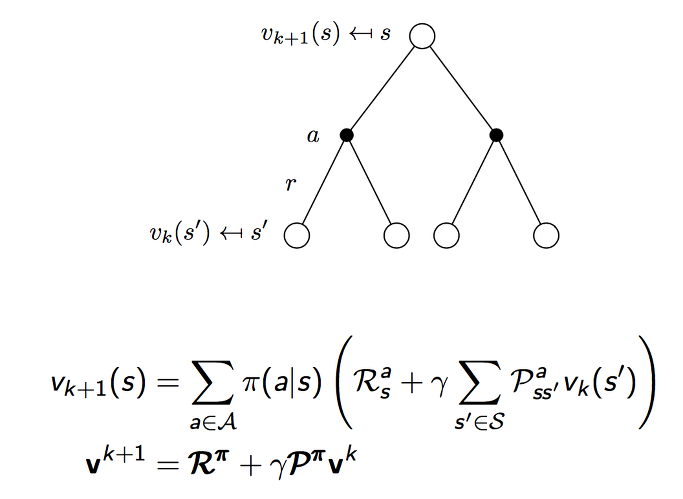
\includegraphics{value_backup}

위 그림에서 k번 째 계산에서 얻은 $v_k(s')$ 들을 사용하여 $v_{k+1}(s)$를 계산하는 
과정을 직관적으로 이해할 수 있어 머리 속에 형상화 시키기가 수월하다. 

위 그림의 예시는 $\pi(a|s)$를 곱하는 과정이 있으므로 정책 이터레이션에 해당한다. 

\section{정책 이터레이션}

정책 이터레이션(반복)은 두 가지 과정을 거친다. 먼저 현재 정책이 얼마나 
좋은 지를 각 상태의 가치를 계산하는 정책 평가가 있고, 여기서 얻은 가치 값에 기초하여 
가장 큰 가치를 돌려주는 행동을 선택하도록 정책의 확률을 조절하는 정책 발전이 있다. 


\subsection{정책 평가} 

정책 평가는 $v_\pi(s)$를 각 상태에 대해 계산하는 것을 뜻한다. 

수식 3.5로 계산을 할 수 있는데 이는 수식 2.32의 벨만 기대 방정식과 약간 차이가 있다. 

수식 3.5: 
$$
v_\pi(s) = \sum_{a \in A} \pi(a|s)(R_{t+1} + \gamma v_\pi(s'))
$$

수식 2.32 계산 가능한 벨만 기대 방정식: 
$$
v_\pi(s) = \sum_{a\in A} \pi(a|s) (R_{t+1} + \gamma \sum_{s' \in S} P_{ss'}^a v_\pi(s'))
$$

수식 3.5에서 수식 2.32에는 있는 전이 확률을 곱하지 않은 이유는 정책에 따라 행동을 결정하면 
무조건 다음 상태 $s'$로 전이된다고 보기 때문이다. 즉, 행동을 선택하면 행동에 대한 다음 상태가 
하나이고 그 확률이 1이라고 본다. 이렇게 보아도 무방하나 그렇지 않은 경우도 있을 수 있으므로 
이 점을 기억해 둔다. 

각 상태의 가치를 나타내는 가치 함수가 2차원 배열 (행렬)에 저장되어 있다. 따라서, 알고리즘은 
$k+1$ 번째 반복 과정에서 $k$ 번째에 저장된 가치 값들로 정책에 따른 선택 확률을 해당 상태로 
전이 되었을 때 얻는 가치와 그 상태의 가치에 곱하여 기대값으로 얻게 된다. 

알고리즘은 책 71 페이지에 상세하게 나와 있다. 각 상태의 $v_{k+1}(s)$는 수식 3.5로 주어지므로 
하나씩 구하여 더하고 행동 선택에 따른 확률을 곱하면 계산할 수 있다. 

초기의 가치 값들은 모두 0에서 시작하고 상태 전이시 보상만 반영하는 것으로 시작하여 
반복이 진행될 때마다 보상 값들도 증가하게 된다. 

\subsection{정책 발전}

정책 발전은 정책 평가가 이루어진 후에 다음 단계의 정책을 결정하는 과정으로 가장 큰 가치를 
주는 행동을 선택하도록 하는 탐욕적 정책을 사용하여 발전 시켜 나가는 것으로 설명하고 있다. 

그리드 월드에서 초기 정책은 모든 행동에 동일한 확률을 부여한 무작위 정책으로 시작하여 
반복할 때마다 가치가 높은 행동을 선택하도록 한다. 이 때 행동별 비교를 위해 행동 가치 함수인 
큐 함수 값을 계산하고 그 결과로 다음 상태를 선택한다. 

수식 3.8 큐 함수의 정의: 
$$
q_\pi(s, a) = \E[R_{t+1} + \gamma v_\pi(S_{t+1}) | S_t = s, A_t = a ]
$$

수식 3.9 계산 가능한 큐 함수 
$$
q_\pi(s, a) = R_s^a + \gamma v_\pi(s')
$$

정책 발전은 최고의 큐 함수 값을 주는 행동을 선택하도록 3.10 처럼 선택한다. 
$$
\pi'(s) = \argmax_{a \in A} q_\pi(s, a)
$$

위의 뜻은 $\pi_{k+1}(s, a) = 1$로 $\argmax$에서 선택한 a에 할당한다는 뜻으로 
다음 부터는 확률 1로 해당 행동을 선택한다는 뜻이다. 

\subsection{종료 조건} 

이와 같이 정책 평가와 정책 발전을 반복하면 최상의 정책 $\pi_*$에 수렴하게 된다. 
이는 증명이 되어 있는데 기본 아이디어는 $q_k(s, a)$ 값이 최고가 되는 값으로 
행동을 선택하므로 $v_k(s)$가 증가하게 되고 이 값은 $v_*(s)$보다는 작으므로 
결국 그 값으로 수렴하게 된다는 것이다. 


그렇다면 정책 반복은 언제 멈추면 될까? 최상의 정책에 도달했다고 판단하면 멈추면 
되는데 이의 근거 중 하나로 정책 평가에서 얻은 가치 함수들의 변화가 거의 없으면 
멈추면 되는 것이 선택 지 중 하나이다. 

\section{가치 이터레이션(반복)}

가치 이터레이션도 최상의 정책 $\pi_*$를 얻기 위해 다이나믹 프로그래밍을 사용하는
알고리즘이다. 가치 반복은 별도의 명시적인 정책을 사용한 정책 반복과 달리 정책이 
가치 함수에 암묵적으로 있다고 보고 최상의 정책을 찾아 나간다. 

정책 발전에서 최상의 가치를 돌려주는 행동을 선택하도록 정책을 개선했으므로 
정책을 사용하지 않고 그냥 최상의 가치를 돌려주는 다음 상태를 직접 선택하는 
암묵적인 정책으로도 최상의 정책을 얻을 수 있다는 것이 핵심 아이디어이다. 

이는 두 가지 수식으로 주어지는 데 하나는 벨만 최적 방정식이고, 다른 하나는 
이를 계산 가능한 형태로 푼 것이다. 

수식 3.13 벨만 최적 방정식 : 
$$
v_*(s) = \max_a \E[R_{t+1} + \gamma v_*(S_{t+1}) | S_t = a, A_t = a]
$$

수식 3.14 계산 가능한 벨만 최적 방정식 : 
$$
v_{k+1}(s) = \max_{a \in A} (R_s^a + \gamma v_k(s'))
$$

가치 반복은 정책이 없으므로 위 과정만으로 각 상태에서 최상의 행동을 알게 된다. 
이는 최상의 다음 상태를 선택하는 행동이므로 정확하게는 최상의 가치를 주는 
다음 상태를 알게 된다는 뜻이다. 

\section{몬테카를로(MC) 예측}

벨만 방정식을 정책 평가와 발전, 가치 반복을 통해 최적의 정책을 찾아가는 
방법을 지금까지 살펴보았다. 이제부터는 실제 경험을 통해 에이전트가 
최적의 가치 함수나 최적 정책을 찾아 나가는 본격적인 강화학습 방법들을 
보는데 그 기초가 MC 예측이다. 

강화학습은 예측과 제어로 이루어지고 예측(Prediction)은 가치 평가에 해당하고 
제어(Control)는 가치 평가나 다른 어떤 기준에 따라 행동을 선택하는 것을 뜻한다. 

강화 학습은 다음과 같은 단계를 밟는다. 

\begin{enumerate}
\item 일단 해보고 
\item (행동의 가치를) 평가하며
\item 평가한 대로 (행동의 선택을) 업데이트하며 
\item 이 과정을 반복한다. 
\end{enumerate}

\subsection{강화학습의 예측과 제어}

상태가 크고 행동에 대한 결과를 모두 알 수 없기 때문에 "적당한 추론"을 통해 
원래 참 가치함수의 값을 예측(Prediction)하고, 예측에 따라 행동을 선택(Control)한다. 

강화학습은 trial and error에 기초한다. 

\subsection{몬테카를로 근사의 예시}

원의 면적 계산을 위해 랜덤한 샘플링을 통해 계산한다. 

$$
\lim_{n \to \infty} \frac{A_n}{B_n} = \frac{S(A)}{S(B)}
$$
$A_n$은 $n$ 번 던졌을 때 A 내부에 있는 건수이고 $B_n$은 B 내부에 있는 건수이다. 

\subsection{샘플링과 몬테카를로 예측}

에이전트(봇)이 환경에서 일련의 보상을 얻는 동작(태스크, 에피소드)을 실행하는 과정이 
하나의 샘플링이다. 샘플링을 많이 반복하여 해당 에피소드 내 상태들이 가치 (상태 가치)와 
행동들의 가치 (상태 행동 가치, Q 함수 값)를 어림으로 추정한다. 

상태 가치 함수 리마인드: $v_\pi(s) = \E[G_t | S_t = s]$

샘플링은 현재 정책에 따라 행동해 보는 과정이다. 이 과정에서 $G_t$를 얻고 
이의 상태별 평균이 $v_\pi$가 된다. 

샘플링은 에피소드로 구성되고, $s_1, a_1, r_1, s_2, a_2, r_2, ... $의 과정으로 
구성된다. 봇이 행동을 선택하여 다음 행동을 하는 것과 같고, 상태는 봇을 포함한 
환경 전체에 있고, 보상은 봇 툴에는 없으나 강화학습에는 필요하다. 

수식 2.32 계산 가능한 벨만 기대 방정식: 
$
v_\pi(s) = \sum_{a\in A} \pi(a|s) (R_{t+1} + \gamma \sum_{s' \in S} P_{ss'}^a v_\pi(s'))
$

위 값을 계산할 때 $\pi(a|s)$와 $P_{ss'}^a$를 알아야 하는데 샘플링 과정에서
알 수가 없기 때문에 샘플링을 통해 얻은 샘플 평균을 근사치로 사용한다. 

$$
v_\pi(s) \approx \frac{1}{N(s)}\sum_{i=1}^{N(s)} G_i(s)
$$

위에서 $N(s)$는 상태 s를 방문한 횟수이고, $G_i(s)$는 상태 s를 방문한 i번째 에피소드의 
반환값 (예상되는 보상)이다. 여기서 $G_i$는 에피소드 전체가 끝나야만 알 수가 있는 값이고 
몬테 카를로 방식의 단점이 된다.  

"수식 4.13 몬테 카를로 예측에서 가치 함수 업데이트의 일반식"이라고 주어진 식이 
이후에도 계속 나오는데 이 과정에 어떤 아이디어가 적용되었는 지를 따라간다. 

\begin{itemize}

\item $V_{n+1}(s) = \frac{1}{n} \sum_{i=1}^n G_i(s) = \frac{1}{n}(G_n(s) + \sum_{i=1}^{n-1} G_i(s))$

위 식을 변형해 나가면 아래 식을 얻는다. 키 아이디어는 $\sum_{i=1}^{n-1} G_i(s) = (n-1)V_n$이 된다는 점이다.

\item $V_{n+1}(s) = V_n(s) ++ \frac{1}{n}(G_n(s) - V_n(s))$

여기서 $n$과 $n+1$ 등은 에피소드 실행마다 증가하는 값이고, 위 식이 $n+1$번째 에피소드를 실행할 때 
계산하는 값이므로 이전의 가치 값을 사용하여 새로운 가치를 계산하는 과정이 된다. 
$V_{n+1}$ 계산에 이전 에피소드의 리턴값인 $G_n$과 이전 에피소드의 가치 값인 $V_n$을 사용한다는 점도 눈여겨 봐야 한다. 

\item $V(s) \leftarrow V(s) + \frac{1}{n}(G(s) - V(s))$

이 식을 역으로 생각하면 최초의 리턴값의 평균이 된다는 점을 기억하자. 

\item $V(s) \leftarrow V(s) + \alpha(G(s) - V(s))$

1보다 작거나 같은 $\alpha$를 스텝 사이즈로 하여 얼마나 새로운 경험에 비중을 둘 지 정한다. 
경험한 리턴값들 사용하여 이와 같이 $V(s)$를 채워 나가면 몬테 카를로를 실행하는 
환경과 에이전트(봇)가 얻게 되는 보상에 수렴하게 된다. 
\end{itemize}

위의 마지막 갱신 수식인 책의 4.13 공식은 이후에도 거의 모두 사용한다. 그래서 위의 
전개 과정을 이해하고 잘 꺼낼 수 있도록 머리에 넣어 두어야 한다. 

\begin{tcolorbox}[title=수식 4.13]
몬테 카를로 예측 이후의 모든 강화학습 방법에서 가치함수를 업데이트 하는 것은 수식 
4.13의 변형일 뿐입니다. 따라서, 이 식을 정확히 이해하는 것이 중요합니다. 

\begin{enumerate}
\item $G(s)=$ 업데이트의 목표 
\item $\alpha(G(s) - V(s))= $ 업데이트의 크기
\end{enumerate}

몬테 카를로 예측에서 에이전트는 이 업데이트 식을 통해 에피소드 동안 경험했던 
모든 상태에 대한 가치함수를 업데이트합니다. 어떠한 상태의 가치함수가 업데이트 될수록 
가치함수는 현재 정책에 대한 참 가치함수에 수렴해갑니다. 

\end{tcolorbox}

\section{시간차 예측 - Temporal Difference Prediction}

몬테 카를로 방법과 달리 에피소드마다가 아닌 타임스텝마다 가치함수를 업데이트하는 
방법이 시간차 예측이다. 이는 사람이 배우는 방식에 더 유사하다. 

시간차 예측에서는 $G_t$를 에피소드 끝까지 더한 값 대신에 다이나믹 프로그래밍의 
정책 평가에서 사용한 방법처럼 전이 상태들의 가치 함수 값을 사용한다. 

$$
v_\pi(s) = \E_\pi[R_{t+1} + \gamma v_\pi(S_{t+1}) | S_t=s]
$$

위 식을 갱신 (업데이트) 방식의 4.13과 같은 수식으로 바꾸면 다음과 같다. 

\begin{tcolorbox}[title=수식 4.17]
$$
V(S_t) \leftarrow V(S_t) + \alpha(R + \gamma V(S_{t+1}) - V(S_t))
$$

\begin{enumerate}

\item $R+\gamma V(S_{t+1}) = $ 업데이트의 목표 

\item $\alpha (R + \gamma V(S_{t+1}) - V(S_t))=$ 업데이트의 크기 

\end{enumerate}

\end{tcolorbox}

위 식에서 $R + \gamma V(S_{t+1}) - V(S_t)$를 시간차 에러(Temporal-Difference Error)라고 한다. 
다른 상태의 가치함수 예측값(이전에 계산한 값)을 통해 지금 상태의 가치 함수를 예측하는 이러한 
방식을 부트스트랩(bootstrap)이라고 한다. 
 
시간차 예측도 참 가치 함수에 수렴하는 것으로 알려져 있다. 

\section{살사 - SARSA}

살사와 Q 러닝은 가치 함수의 값을 찾아가는 예측과 가치 함수에 따라 행동을 선택하는 제어를 
모두 포함하는 본격적인 강화학습 알고리즘이고 모든 가치 기반 강화학습의 기초가 되는 
알고리즘이다. 따라서, 지금까지 이해해 온 바로 살사와 큐 러닝까지 이해하면 테이블 기반 
강화학습의 기초가 마련되었다고 할 수 있다. 

살사는 에이전트가 경험하는 샘플 $[S_t, A_t, R_{t+1}, S_{t+1}, A_{t+1}]$을 통해 
큐 함수 값을 업데이트하고, 이 큐 함수에 기반하여 행동을 선택하면서 시뮬레이션을 
진행하여 최적의 큐 함수를 통해 최적의 정책을 찾아가는 알고리즘이다. 

큐 함수를 이용하는 이유는 정책인 $\pi(a|s)$ 또는 $P_{ss'}^a$를 모르는 상태에서 
최적의 행동을 찾아가야 하기 때문인데, 다음 행동을 $\pi(s) = \argmax_{a \in A} Q(s, a)$로 
찾는다. 이런 정책을 탐욕 정책 (greedy policy)라고 하는데 항상 최고의 보상을 돌려주는 
행동을 하기 때문에 약간 게걸스럽게 먹는 모습이 떠올라 붙인 이름으로 보인다. 

탐욕 정책을 사용하면 AI의 근본 문제라고 할 수 있는 탐색(exploration)과 활용(exploitation)의 
균형이 시뮬레이션 초기에는 깨져서 더 나은 정책이 있음에도 항상 이전에 최고의 보상을 
준 행동에서 멈추는 현상이 생기게 된다. 이를 보완하는 가장 기본적인 방법으로 
$\epsilon$-탐욕 ($\epsilon$-greedy) 정책을 사용한다. 이는 $\epsilon$의 확률만큼 
랜덤하게 행동을 선택하여 탐색을 일정 비율로 지속하게 한다. (수식 4.21 참고)

이와 같이, 정책 반복에서 본 것처럼 탐색과 활용을 큐 함수를 갱신하면서 점점 
최적의 정책에 다가가는 방법이 살사이다. 

큐 함수의 업데이트는 수식 4.20으로 주어진다. 
$$
Q(S_t, A_t) \leftarrow Q(S_t, A_t) + \alpha(R_{t+1} + \gamma Q(S_{t+1}, A_{t+1}) - Q(S_t, A_t))
$$

\subsection{살사 코드 설명}

살사 코드는 이제 본격적인 테이블 기반 강화 학습 방법을 설명하는 코드이고 
골격이 Q 러닝과 비슷하기 때문제 살펴볼 가치가 있다. 

코드는 SARSAgent, Env, 에피소드 실행 세 가지로 구성된다. 

SARSAgent는 q\_table, actions를 갖고 있고, learning\_rate ($\alpha$), 
discount\_factor ($\gamma$), epsilon($\epsilon$-greedy)을 초기화 한다. 

learn 함수는 수식 4.20으로 새로운 큐 값을 갱신한다. 

get\_action은 $\epsilon$ 탐욕 정책을 어떻게 구현하는 지 보여주고
arg\_max가 최대 큐 값을 갖는 액션을 돌려주는 함수이다. 

에피소드 실행은 1000번 하고, 각 에피소드는 에이전트의 초기 상태에서 
행동을 실행하고, 다음 상태와 보상 값을 갖고 학습 하면서 반복한다. 

실제 봇툴에 구현할 때 환경의 상태 구현을 어떻게 할 지가 매우 
중요하다는 것을 env.reset(), evn.step() 함수의 내부 구현에 대해 
생각해 보면 알 수 있다. 

\section{큐러닝}

\subsection{살사의 한계}

살사의 한계를 분석할 때 사용하는 개념은 온폴리시와 오프폴리시 개념은 중요하다. 
온폴리시는 최적화를 위해 찾아가는 정책과 행동을 선택하는 정책이 같다는 뜻이고, 
오프폴리시는 최적화 정책과 행동을 결정하는 정책이 다르다는 뜻이다. 

살사의 한계가 비롯된 이유는 $\epsilon$ 탐욕 정책을 최적화에 그대로 사용했기 
때문에 한번 잘못도니 길을 선택하게 되면 그 보상 값도 반영되기 때문에 
이후에도 낮은 값의 큐 함수로 남아 있어 해당 행동이 최적이 될 수 있음에도 
선택을 못 하게 되는 경우가 생기기 때문이다. 

큐 러닝은 오프폴리서 알고리즘으로 $\epsilon$ 탐욕 정책으로 다음 행동을 
선택하기는 하나 큐 함수의 값 업데이트는 최적의 값을 사용한다는 차이가 있다. 
이렇게 최적 정책을 찾아가는 정책과 행동을 선택하는 정책이 차이가 있어 
오프폴리시 알고리즘이라고 한다. 

큐 러닝에서 큐 함수의 업데이트 수식은 4.24로 주어진다. 

$$
Q(S_t, A_t) \leftarrow Q(S_t, A_t) + \alpha(R_{t+1} + \gamma \max_{a'} Q(S_{t+1}, a') - Q(S_t, A_t))
$$

이는 벨만 최적 방정식 2.41과 같다. 

$$
q_*(s, a) = \E[R_{t+1} + \gamma \max_{a'} q_*(S_{t+1}, a') | S_t = s, A_t = a]
$$

\subsection{큐러닝 코드 설명}

살사와 코드 구조가 거의 차이가 없고, learn 함수만 다르다. 

learn 함수에서 벨만 기대 방정식으로 큐 함수를 업데이트 하는 대신에 
벨만 최적 방정식으로 큐 함수를 업데이트 한다. 이는 현재 선택한 
행동 (정책) 대신에 최적의 행동(오프 폴리시)을 사용하는 효과를 만든다. 

\section{큐러닝 연습 - 택시}

https://ichi.pro/ko/openai-gymeul-tonghan-q-learning-sogae-49999016693565

openAI gym은 강화학습 알고리즘 테스트에 많이 쓰이는 강화학습 환경이다. 
파이썬에서 pip로 설치할 수 있으며 큐러닝 소스들도 많이 있다. 

위의 링크를 보고 따라서 해보면서 잘 되는 지, 어떻게 학습하는 지 확인한다. 

이번 기회에 numpy 등 파이썬 라이브러리를 일부 공부하고 gym을 살펴보도록 한다. 

\section{큐러닝 연습 - 테트리스}

https://github.com/nuno-faria/tetris-ai

위 링크는 신경망을 사용한 Deep RL로 테트리스 플레이를 구현한 예시이다. 
이를 테이블 기반 큐러닝으로 변경하여 구현한다. 변경하여 구현하면서 
한번 NN(신경망) 코드를 만나게 된다.  


\section{근사함수}

\subsection{몬테카를로, 살사, 큐러닝의 한계}

테이블 기반 강화학습 알고리즘들은 상태가 커지거나 선택할 수 있는 행동이 
많아지면 계산 불가능하거나 메모리에 저장할 수 없을 정도로 차원이 커지게 되어 
실제 문제에 적용이 매우 어렵게 된다. 

이런 한계를 극복하기위해 가치함수(큐함수)의 저장을 근사시켜서 신경망에 
저장하도록 학습시키고 다시 꺼내서 사용하는 접근이 많이 사용되고 있으며 
이를 심층강화학습(Deep RL)이라고 한다. 

\subsection{근사함수를 통한 가치함수의 매개변수화}

책에서 그림 5.3의 데이터를 매개변수를 4개로 하는 3차 함수로 근사 시키는 
예시가 있다. $y=ax^3 + bx^2 + cx + d$에서 $(a, b, c, d)$ 값이 매개변수가 되고 
복잡한 정보를 네 개의 정보로 근사시키게 된다. 

이와 같이 차원이 높은 복잡한 데이터를 근사 시키는 능력이 신경망에 있어 
인공 신경망을 사용하여 근사 시키는 방법을 사용하고 이와 같은 방법이 
강화학습에서도 많이 연구되어 있다. 


\section{인공신경망}

\subsection{Math Behind DNN}

https://towardsdatascience.com/https-medium-com-piotr-skalski92-deep-dive-into-deep-networks-math-17660bc376ba

시각화로 간단하게 왜 동작하는 지 느낌을 얻도록 도와준다. 



\end{document}
























